\documentclass[a4paper, 8pt]{extarticle}

\usepackage[greek,spanish,es-tabla,es-nodecimaldot]{babel}
\usepackage[a4paper, lmargin=0.2cm,rmargin=0.2cm,tmargin=1cm,bmargin=1cm, landscape]{geometry}
\usepackage{multicol}
\usepackage{amsmath}
\usepackage{mathtools}
\usepackage[exponent-product = \cdot, per-mode = fraction]{siunitx}
\usepackage{cancel}

\usepackage{siunitx}
\DeclareSIUnit\octave{oct}
\DeclareSIUnit\decade{dec}
\sisetup{
    inline-per-mode = symbol
}

\usepackage{physics}
\AtBeginDocument{\RenewCommandCopy{\qty}{\SI}}

\usepackage{lipsum}
\usepackage{esvect}
\renewcommand{\vec}[1]{\vv{{#1}}}
\renewcommand{\grad}{\vec{\nabla}}
\renewcommand{\cot}{\operatorname{cotg}}

\usepackage{parskip}
\usepackage{tabu}

\usepackage{tikz}
\usetikzlibrary{arrows, babel, fadings}

\usepackage{circuitikz}
\ctikzset{bipoles/length=1cm}

\usepackage{lmodern}
% \renewcommand{\familydefault}{\sfdefault}
% \renewcommand{\rmdefault}{\sfdefault}

\usepackage{titlesec}
\titleformat{\section}
{\color{blue}\normalfont\Large\bfseries}{\thesection}{1em}{}[{\titlerule[0.8pt]}]
\titleformat{\subsection}{\normalfont\large\bfseries}{\thesubsection}{1em}{}

\titlespacing*{\section}{0pt}{12pt plus 4pt minus 2pt}{5pt plus 2pt minus 2pt}
\titlespacing*{\subsection}{0pt}{12pt plus 4pt minus 2pt}{3pt plus 2pt minus 2pt}
\titlespacing*{\subsubsection}{0pt}{12pt plus 4pt minus 2pt}{3pt plus 2pt minus 2pt}

%\allowdisplaybreaks
\setcounter{secnumdepth}{-1}
\setcounter{tocdepth}{-1}

\newcommand{\pag}[1]{\text{(Pág. #1)}}
\DeclareSIUnit\rayl{rayl}
\DeclareSIUnit\dbspl{\text{dB\ensuremath{_{\textup{SPL}}}}}
\DeclareSIUnit\dbsil{\text{dB\ensuremath{_{\textup{SIL}}}}}


%%% INICIO DEL DOCUMENTO %%%
\begin{document}
\setlength{\parskip}{0pt}
\setlength{\parindent}{0pt}
\pagestyle{empty}
\renewcommand{\arraystretch}{1.5}

\begin{multicols}{3}
    \section{Glosario}
    \[
        \begin{alignedat}{2}
            S          & \equiv \text{Sensibilidad}  \left[ \unit{\dbspl} \right]                                                  \\
            H          & \equiv \text{Función de transferencia}  \left[ \unit{\dB} \text{ re. }\unit{\volt\per\pascal} \right]     \\
            P          & \equiv \text{Potencia} \left[ \unit{\watt} \right]                                                        \\
            V          & \equiv \text{Tensión en bornes del altavoz (a veces aparece como } E \text{)} \left[ \unit{\volt} \right] \\
            \text{SPL} & \equiv \text{Nivel de presión sonora (a veces aparece como } L \text{)} \left[ \unit{\dbspl} \right]      \\
            Z_n        & \equiv \text{Impedancia nominal del altavoz} \left[ \unit{\ohm} \right]                                   \\
            Q          & \equiv \text{Factor de sobrecarga (o factor de calidad en circuitos eléctricos)}                          \\
        \end{alignedat}
    \]

    \section{Fórmulas útiles}
    \subsection{Nivel de presión en la banda útil}
    \[
        \text{SPL}_{\Delta \textup{B}} = 10 \log \left( \sum_{i}^{N} 10^{\frac{\text{SPL}_i}{10}} \right)
    \]
    \color{gray}\begin{itemize}
        \item $\Delta \textup{B}$ se refiere a la banda de frecuencias en la que se realiza la suma (generalmente el rango útil del altavoz).
        \item $N$ es el número de bandas.
    \end{itemize}\color{black}

    \subsection{Potencia en la banda útil}
    La potencia se puede sumar directamente:
    \[
        P_{\Delta \textup{B}} = \sum_{i}^{N} P_i
    \]

    \subsection{Décadas y octavas}

    Un filtro con pendiente de \qty{6}{\dB \per \octave} tiene una pendiente de \qty{20}{\dB \per \decade}.
    \[ \begin{alignedat}{3}
            \text{Década:}       & \quad & f_2 & = 10 f_1        \\
            \text{Octava:}       &       & f_2 & = 2 f_1         \\
            \text{Media década:} &       & f_2 & = \sqrt{10} f_1
        \end{alignedat} \]


    \section{Parámetros de altavoces}

    \subsection{Impedancia nominal}
    Esta impedancia $Z_n$ es un valor real que sustituye a la impedancia eléctrica equivalente $Z_{ee}$ del altavoz para los cálculos eléctricos, ya que esta última es compleja y depende de la frecuencia. \color{gray} Se debe cumplir que $\abs{Z_{ee}(f)} \geq 0.8 Z_n$. \color{black}

    \subsection{Potencia disipada en el altavoz}
    Usando la ley de Ohm ($V=I \cdot R$), la potencia queda como:
    \[ P = V \cdot I = \frac{V^2}{Z_n}\]
    \color{gray}
    Donde $I$ es la corriente que circula por el altavoz (apenas se usará para los primeros temas de SEA).
    \color{black}

    \subsection{Sensibilidad}
    La sensibilidad $S$ de un altavoz se define como el nivel de presión sonora radiada por el altavoz cuando se le excita con una potencia de \qty{1}{\watt}, sobre la impedancia nominal, a \qty{1}{\meter} de distancia y en el eje de máxima radiación.

    \[ S \left( \qty{1}{\watt }, \qty{1}{\meter }, \qty{0}{\degree } \right) = 20 \log \left( \frac{p _{\text{eje}}}{p _{\text{ref}}} \right)  \]

    \subsubsection{Corrección de la distancia y de la potencia}
    Si la distancia a la que se mide la sensibilidad no es de \qty{1}{\meter} o si la potencia aplicada en la banda útil no es de \qty{1}{\watt}, se puede calcular la sensibilidad como:
    \[
        S \left( \qty{1}{\watt }, \qty{1}{\meter}, \qty{0}{\degree }  \right) = \text{SPL}_{r,P} + 20 \log \left( r \right) - 10 \log \left( P \right)
    \]

    \color{gray}Donde $\text{SPL}_{r,P}$ es el nivel de presión sonora medido a una distancia $r$ tras aplicar una potencia $P$ al altavoz en la banda útil.\color{black}

    \subsection{Función de transferencia}

    La función de transferencia $H$ de un altavoz se define como la relación entre la tensión en los bornes del altavoz y la presión sonora radiada por el altavoz.
    \[ H = 20 \log \left( \frac{p_{\text{eje}}}{V} \right)  \]

    \subsection{Método de Small}

    El método de Small es un método de cálculo de los parámetros Thiele-Small a partir de la impedancia eléctrica equivalente $Z_{ee}(f)$ del altavoz. A partir de la gráfica de $\abs{Z_{ee}(f)}$ con respecto a la frecuencia, los pasos son:
    \begin{enumerate}
        \item Calcular $R_e$ como el valor de $\abs{Z_{ee}(f)}$ en $f=\qty{0}{\Hz}$, o en la frecuencia más baja que aparezca.
        \item Calcular $Z _{\text{res}}$ como $\max \left\lbrace \abs{Z_{ee}(f)} \right\rbrace $, es decir, el valor del pico de resonancia. Así obtenemos también $f _{\text{res}}$, que es la frecuencia en la que se da este pico.
        \item Calcular $r_0$ y $Z_{r_0}$ según las fórmulas de la tabla.
        \item Dibujamos una línea recta horizontal en el gráfico a la altura de $Z_{r_0}$. Los puntos de corte con la curva alrededor de la resonancia nos dan $f_1$ y $f_2$.
        \item Ya podemos calcular los factores de sobrecarga según las fórmulas de la tabla.
    \end{enumerate}
    \begin{center}
        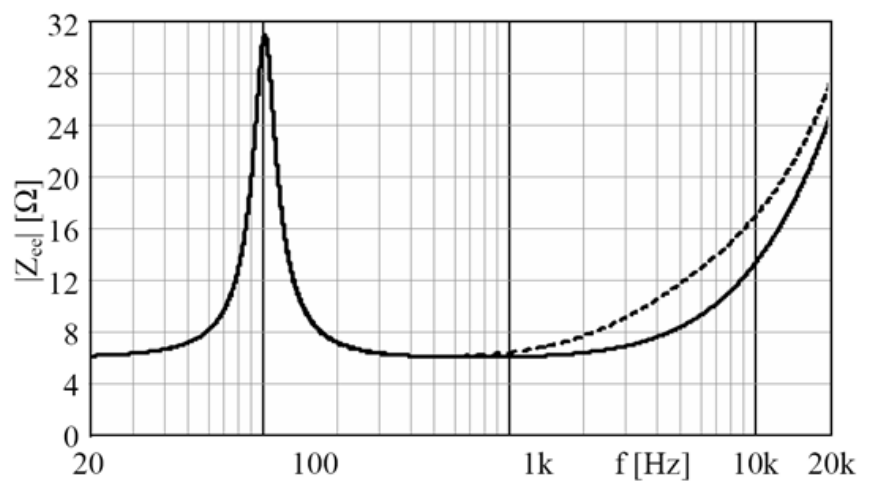
\includegraphics[width=0.7\linewidth]{images/Zeq.png}
    \end{center}

    \subsection{Parámetros de Thiele-Small}
    \begin{center}
        \begin{tabular}{|c|c|l|}
            \hline
            \textbf{Param}         & \textbf{SI}     & \textbf{Descripción y valor}                                                                  \\
            \hline
            $R _{\text{dc}} / R_e$ & \unit{\ohm}     & Resistencia total del circuito en continua                                                    \\
            $f _{\text{res}}$      & \unit{\hertz}   & Frecuencia de resonancia                                                                      \\
            $M _{\text{ms}}$       & \unit{\kg}      & Masa móvil                                                                                    \\
            $C _{\text{ms}}$       & \unit{\meter}   & Compliancia mecánica del diafragma                                                            \\
            $S_d$                  & \unit{\meter^2} & Superficie efectiva del diafragma                                                             \\
            $Z _{\text{res}} $     & \unit{\ohm}     & Impedancia a la frecuencia de resonancia                                                      \\
            $r_0$                  & -               & $r_0 =\frac{Z _{\text{res}}}{R_e}$                                                            \\
            $Z_{r_0}$              & \unit{\ohm}     & $Z_{r_0}=R_e \sqrt{r_0}$                                                                      \\
            $f_1, f_2$             & \unit{\hertz}   & Frecuencias para calcular los factores $Q$                                                    \\
            $Q _{\text{ms}}$       & -               & Factor de sobrecarga mecánico $Q _{\text{ms}} = \frac{f _{\text{res}} \sqrt{r_0}}{f_2 - f_1}$ \\
            $Q _{\text{es}}$       & -               & Factor de sobrecarga eléctrico $Q _{\text{es}} = \frac{Q _{\text{ms}}}{r_0 - 1}$              \\
            $Q _{\text{ts}}$       & -               & Factor de sobrecarga total $Q _{\text{ts}} = \frac{Q _{\text{ms}}}{r_0}$                      \\
            \hline
        \end{tabular}
    \end{center}

    \vfill\null
    \columnbreak

    \section{Filtros de cruce (\textit{crossover filters})}

    \subsection{Red de Zobel}
    Como los filtros de cruce se diseñan considerando que la impedancia del altavoz es la impedancia nominal, el comportamiento real del filtro difiere del calculado, principalmente debido a:

    \begin{itemize}
        \item Resonancia mecánica del altavoz.
        \item Autoinducción de la bobina a altas frecuencias.
    \end{itemize}
    Las redes de Zobel ayudan a ``aplanar'' la impedancia del altavoz. Este problema solo afecta a filtros pasivos.

    \subsection{Variable de Laplace normalizada}
    Es habitual encontrar los filtros definidos por su función de transferencia con la variable $s$ normalizada. A menudo se da por hecho y no la distinguen, pero lo adecuado es definirla con otro nombre, así:
    \[s_0 = \frac{s}{\omega_c} = \frac{s}{2 \pi f_c}\]

    \subsection{Filtros de Butterworth}

    Presentan potencia constante $\left( \abs{H_P (\omega)}^2 = \abs{H_L (\omega )}^2 + \abs{H_H (\omega )}^2   = 1\right)$, pero no tensión constante (excepto el de orden 1). La frecuencia de corte se define a \qty{-3}{\dB}.

    \subsubsection{Polinomios de Butterworth}
    \begin{align*}
        B_1(s)  & = s + 1                                                                                             \\
        B_2(s)  & = s^2 + \sqrt{2} s + 1                                                                              \\
        B_3(s)  & =  \left( s+1 \right)\left( s^2 +s+1 \right) \color{gray} = s^3 + 2 s^2 + 2 s + 1 \color{black}     \\
        B_4(s)  & = \left( s^2 +1.848 s +1 \right) \left( s^2 +0.7654s +1 \right)                                     \\
        B_5(s)  & = \left( s + 1 \right) \left( s^2 + 1.618s + 1 \right) \left( s^2 + 0.618s + 1 \right)              \\
        B_6 (s) & = \left( s^2 + 1.932s + 1 \right) \left( s^2 + \sqrt{2}s +1 \right) \left( s^2 +0.5176s + 1 \right)
    \end{align*}

    \subsection{Filtros de Linkwitz-Riley}

    Son el producto de dos filtros Butterworth.
    \[ L_{2r}(s) = \left[ B_r (s)\right]^2 \]

    \subsubsection{Polinomios de Linkwitz-Riley}
    \begin{align*}
        L_2 (s) & = \left( s + 1 \right)^2               \\
        L_4 (s) & = \left( s^2 + \sqrt{2}s + 1 \right)^2 \\
        L_6 (s) & = \left( s^3  +2s^ 2 +2s +1 \right)^2  \\
    \end{align*}
    % \vfill\null
    % \columnbreak
\end{multicols}
\end{document}
